\documentclass[10pt,a5paper]{extarticle}
\usepackage[margin=1cm]{geometry}
\usepackage[utf8]{inputenc}
\usepackage[IL2]{fontenc}
\usepackage[czech]{babel}
\usepackage{microtype}
\usepackage{amssymb}
\usepackage{amsthm}
\usepackage{amsmath}
\usepackage{xcolor}
\usepackage{graphicx}
\usepackage{wasysym}

\usepackage[inline]{enumitem}

\newcommand{\R}{\mathbb{R}}

\newcommand{\hint}[1]{{\color{gray}\footnotesize\noindent(Nápověda: #1)}}

\setlist[enumerate]{label={(\alph*)},topsep=\smallskipamount,itemsep=\smallskipamount,parsep=0pt}
\setlist[itemize]{topsep=\smallskipamount,noitemsep}

\def\tisk{%
\newbox\shipouthackbox
\pdfpagewidth=2\pdfpagewidth
\let\oldshipout=\shipout
\def\shipout{\afterassignment\zdvojtmp \setbox\shipouthackbox=}%
\def\zdvojtmp{\aftergroup\zdvoj}%
\def\zdvoj{%
    \oldshipout\vbox{\hbox{%
        \copy\shipouthackbox
        \hskip\dimexpr .5\pdfpagewidth-\wd\shipouthackbox\relax
        \box\shipouthackbox
    }}%
}}%



\newtheorem*{poz}{Pozorování}

\theoremstyle{definition}
\newtheorem{uloha}{\atr Úloha}
\newtheorem{suloha}[uloha]{\llap{$\star$ }Úloha}
\newtheorem*{bonus}{Bonus}
\newtheorem*{defn}{Definice}

\pagestyle{empty}

\DeclareMathOperator{\arctg}{arctg}
\DeclareMathOperator{\tg}{tg}

\let\=\doteq
\let\ee\expandafter

\def\vysld{}
\let\printvysl\relax
\let\printalphvysl\relax

\makeatletter
\long\def\vyslplain#1{\ee\ee\ee\gdef\ee\ee\ee\vysld\ee\ee\ee{\ee\vysld\ee\printvysl\ee{\the\c@uloha}{#1}}}

\def\locvysl#1{\ee\gdef\ee\locvysld\ee{\locvysld\item #1}}
\let\lv\locvysl

\newenvironment{ulohav}[1][]{\begin{uloha}[#1]\gdef\locvysld{\begin{enumerate}}}{\ee\vyslplain\ee{\locvysld\end{enumerate}}\end{uloha}}

\makeatother

\def\atr{}
\def\basic{\def\atr{\llap{\mdseries$\sun$ }\gdef\atr{}}}
\def\interest{\def\atr{\llap{$\star$\,}\gdef\atr{}}}

\begin{document}

%\tisk

\section*{6. Rozlučka s tělesy}

%Ve všech úlohách značí $S_{XY}$ střed úsečky $XY$.

%\the\mathcode`\,
\mathcode`\,="013B

%\basic


%\basic
\begin{uloha}
Olovo má za pokojové teploty hustotu $11,34\,\mathrm{g}\cdot\mathrm{cm}^{-3}$, ovšem při zkapalnění hustota poklesne na $10,66\,\mathrm{g}\cdot\mathrm{cm}^{-3}$. Jaký poloměr má mít kulová kapka kapalného olova, abychom po ztuhnutí dostali kulku o poloměru 0,5\,cm?\vyslplain{$0,5 \sqrt[3]{\frac{11,34}{10,66}} \doteq 0,5104\,\mathrm{cm}$}
\end{uloha}


\basic
\begin{uloha}
Jaký povrch má jehlan, jehož podstavou je obdélník o rozměrech $50 \times 78$ a délka boční hrany je $65$?\vyslplain{10956}
\end{uloha}


\begin{ulohav}
Bruno v laboratoři naklonil těleso $\mathfrak T$ plné kyseliny o $30^\circ$, čímž se z něj část kyseliny vylila. Určete, jaký objem kyseliny v $\mathfrak T$ zůstal, pokud $\mathfrak T$ je
\begin{enumerate}
    \item krychle o hraně délky $1$,\lv{$1-\frac{\sqrt{3}}{6}\doteq 0,711$}
    \item polokoule o poloměru $1$ (otočená plochou stranou nahoru).\lv{$\frac5{24}\pi \doteq 0,6545$}
\end{enumerate}
\end{ulohav}

\basic
\begin{uloha}
Osovým řezem válce je čtverec o obsahu $25$. Vypočítejte povrch válce.\vyslplain{$\frac{75}{2}\pi$}
\end{uloha}

%\basic
\begin{uloha}
Určete, kolik procent koule zabírá největší možný kužel, který se do té koule vejde, a má odchylku strany od podstavy $75^\circ$.
\hint{Poloměr koule lze efektivně zjistit pomocí \uv{rozšířené verze} sinové věty.}\vyslplain{cca 11,663\,\%}
\end{uloha}

\interest
\begin{uloha}
Vyřešte předchozí úlohu pro obecný úhel $\alpha$ namísto $75^\circ$.\vyslplain{$\frac{1}{4} \sin ^3(2\alpha) \tg \alpha = 2 \cos^2 \alpha \sin^4 \alpha$}
\end{uloha}

\interest
\begin{uloha}
Plastový pivní kelímek má tvar komolého kužele o poloměrech podstav 4\,cm a 5\,cm 
a výšce 8\,cm. V kelímku zbývá 0,25\,l piva. Jak vysoko dosahuje hladina piva? (Pokud vás nenapadne jistý celkem trik, tak jen sestavte vhodnou rovnici a vyřešte ji numericky pomocí softwaru.)\vyslplain{cca 4,54428\,cm}
\end{uloha}

\interest
\begin{uloha} % Náboj 2014
Mezi tři stejné kužely, které stojí na podložce tak, že se navzájem dotýkají podstavami, jsme vložili kouli. Koule je tak velká, že její nejvyšší bod leží ve stejné výšce jako vrcholy kuželů. Kužely mají podstavu o poloměru 50\,cm a jejich výška je 120\,cm. Zjistěte poloměr koule.\vyslplain{$\frac{200\sqrt3}{9}$}
\[ 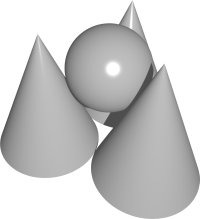
\includegraphics[width=4cm]{gula_medzi_kuzelmi.png} \]
\end{uloha}

\newpage
\parindent=0pt
\parskip=\smallskipamount
\def\printvysl#1#2{\textbf{#1.}\ #2\par}
\vysld

\end{document}